%%%%%%%%%%%%%%%%%%%%%%%%%% ch3
\begin{frame}
  \frametitle{主要内容}
  \tableofcontents[hideallsubsections]
\end{frame}

\section{准备知识}
\begin{frame}
\begin{theorem}
	如果函数$f(x)$在区间$[a,b]$上连续,则积分上限函数
	\[\Phi(x)=\int_a^x f(t)dt\]
	在[a,b]上具有导数,并且它的导数是
	\[\Phi^\prime(x)=\frac{d}{dx}\int_a^xf(t)dt=f(x)\qquad (a\le x\le b) \]
\end{theorem}
\begin{theorem}
	如果函数$f(x)$在区间$[a,b]$上连续,则函数
	\[\Phi(x)=\int_a^x f(t)dt\]	
	就是$f(x)$在$[a,b]$上的一个原函数。
\end{theorem}
\end{frame}

\begin{frame}
\begin{theorem}
	如果函数$F(x)$是连续函数$f(x)$在区间$[a,b]$上的一个原函数,则
	\[\int_a^b f(x)dx=F(b)-F(a)\]	
\end{theorem}
\end{frame}

\section{统计检测基本模型}

\begin{frame}{术语(1)}
\textcolor{red}{$H_j(j=0,1)$: 信源输出的信号, 称为假设$H_j$}

\bigskip

\textcolor{red}{$P(H_j)(i=0)$: 假设$H_j$为真的先验概率(先验:先于试验)}


\bigskip
\textcolor{red}{$(x|H_j)(j=0,1)$: 假设$H_j$下的观测信号是随机变量}

\bigskip

\textcolor{red}{$p(x|H_j)(j=0,1)$: 假设$H_j$下观测信号的概率密度函数}

\bigskip

\textcolor{red}{$(H_i|H_j)(i,j=0,1)$: 在假设$H_j$为真的条件下,判决假设$H_i$成立的结果。}\\
~\\
\textcolor{red}{$P(H_i|H_j)(i,j=0,1)$: 在假设$H_j$为真的条件下,判决假设$H_i$成立的概率。}\\
~\\
\textcolor{red}{$c_{ij}$: 在假设$H_j$为真的条件下,判决假设$H_i$成立所付出的代价。}
 
\end{frame}

\begin{frame}{贝叶斯判决准则}
\textcolor{blue}{\textbf{判决表达式}}
\[
\lambda(x)\mathop{\gtrless}_{H_0}^{H_1}\eta
\]

\[ \lambda(x)\mathop{=}\limits^{def}\frac{p(x|H_1)}{p(x|H_0)} \] \textcolor{blue}{定义为\textbf{似然比函数}}

\bigskip
\[\eta\mathop{=}\limits^{def}\frac{P(H_0)(c_{10}-c_{00})}{P(H_1)(c_{01}-c_{11})} \] \textcolor{blue}{定义为\textbf{判决门限}}

\bigskip
\textcolor{blue}{\textbf{化简}(例如对数似然比检验)}
\[
\ln\lambda(x)\mathop{\gtrless}_{H_0}^{H_1}\ln\eta
\]

\end{frame}

\begin{frame}{M元信号检测模型}
\[\bm{R}=\bigcup\limits_{i=0}^{M-1}R_i, \quad R_i\cap R_j=\emptyset,(i\ne j) \]

\bigskip

\colorbox{yellow}{最佳信号检测$\Leftarrow$正确划分观测空间$\bm{R}$中的各个判决域$R_i\Leftarrow$最佳检测准则} 

\bigskip

\textcolor{blue}{\textbf{两种假设先验等概$\implies P(H_0)=P(H_1)=\frac{1}{2}$}}

\bigskip


\tiny{
\colorbox{yellow}{采样样本$x_i(i=1,2,\dots,N)$之间相互统计独立, 因此其$N$维联合概率密度能够表示成各自一维概率密度之积的形式, 即}\\
}

\colorbox{yellow}{$p(x_1,x_2,\dots,x_N)=p(x_1)p(x_2)\cdots p(x_N)=\prod\limits_{i=1}^Np(x_i)$} 
\end{frame}

\begin{frame}[shrink]
\begin{block}{思考}
	如果$n$是均值为零的, 方差为$\sigma_n^2$的高斯随机变量, 两个假设下的观测信号模型\\
	$H_1: r=1+n$\\
	$H_0: r=-1+n$\\
	观测信号$p(r|H_1),p(r|H_0)$应服从何种分布?
\end{block}
\begin{block}{}
	因为高斯随机变量的特点:高斯随机变量的线性组合还是高斯随机变量。\\
	习题2.7: $x\sim\mathcal{N}(\mu_x,\sigma_x^2)$,则$(y=ax+b)\sim\mathcal{N}(a\mu_x+b,a^2\sigma_x^2)$。\\
	所以, $p(r|H_1)\sim\mathcal{N}(1,\sigma_n^2)$, $p(r|H_0)\sim\mathcal{N}(-1,\sigma_n^2)$
\end{block}
\begin{block}{}
	直接计算: $E(r|H_0)=E(1+n)=1+E(n)=1,Var(r|H_0)=E[(r|H_0-E(r|H_0))^2]=E[n^2]=\sigma_n^2\implies r|H_0\sim\mathcal{N}(1,\sigma_n^2)$\\
	$E(r|H_1)=E(-1+n)=-1+E(n)=-1,Var(r|H_1)=E[(r|H_1-E(r|H_1))^2]=E[n^2]=\sigma_n^2\implies r|H_1\sim\mathcal{N}(-1,\sigma_n^2)$
\end{block}
\end{frame}

\begin{frame}
\begin{columns}
	\column{0.4\textwidth}
	\begin{align*}
	&&n\sim\mathcal{N}(0,\sigma^2)\\ 
	H_0 &:x=n   &x\sim\mathcal{N}(0,\sigma^2)\\
	H_1 &:x=m+n &x\sim\mathcal{N}(m,\sigma^2)\\
	\end{align*}
	\[\text{判决表达式:  } x\mathop{\gtrless}_{H_0}^{H_1}\frac{\sigma^2}{m}\ln\eta+\frac{m}{2} \]
	\column{0.4\textwidth}
	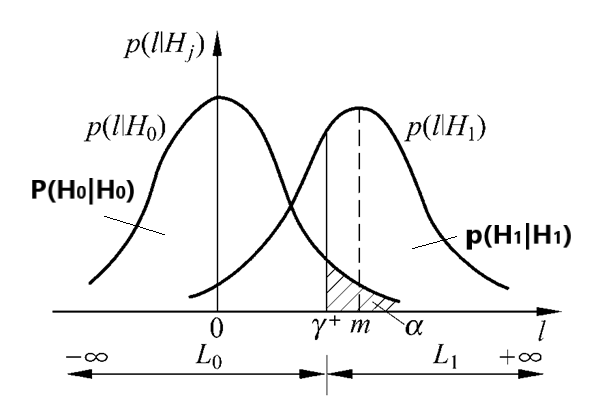
\includegraphics[scale=0.3]{mgt0}\\
	\scriptsize
	\textcolor{blue}{$p(l|H_j)(j=0,1)$: 假设$H_j$下观测信号的概率密度函数; $r^+=\frac{\sigma^2}{m}\ln\eta+\frac{m}{2}; \alpha=P(H_1|H_0)$}
\end{columns}
\begin{block}{思考}
	\begin{enumerate}
		\item $\frac{m}{2}$是两个假设的中间值, $\frac{\sigma^2}{m}\ln\eta$为中间值的修正量, 其含义如何?
		\item 考虑$m>0,m<0,m=0$时,如何构造判决表达式?
	\end{enumerate} 
\end{block}
\end{frame}

\begin{frame}
\begin{enumerate}
	\item $m=0$时: $H_0,H_1$成为一样的信号。
	\item $m\uparrow\implies$ 中间值修正量$(\frac{\sigma^2}{m}\ln\eta)\downarrow$, $r$越接近于中间值$\frac{m}{2}$。
	\item $m$值越大, 更易区分两种假设,检测性能越好。
	\item $m>0$和$m<0$下的判决表达式如下图。
\end{enumerate}	
\begin{columns}
	\column{0.4\textwidth}
	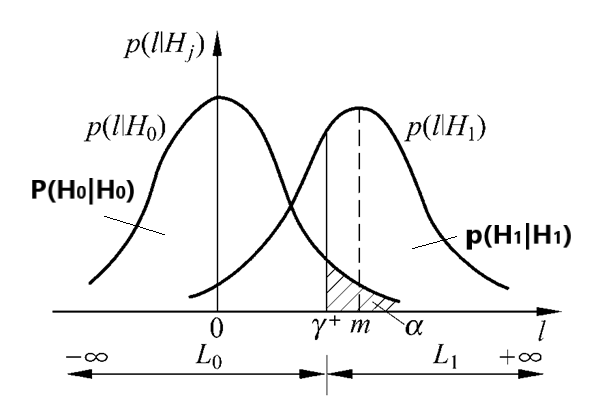
\includegraphics[scale=0.3]{mgt0}
	$m>0;\qquad x\mathop{\gtrless}\limits_{H_0}^{H_1}\frac{\sigma^2}{m}\ln\eta+\frac{m}{2}$
	\column{0.4\textwidth}
	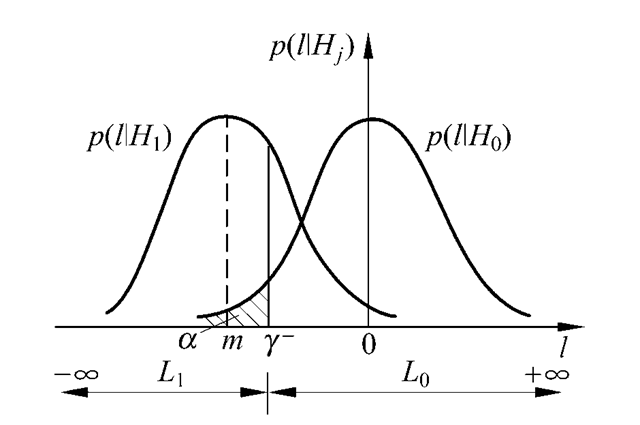
\includegraphics[scale=0.45]{mle0}
	$m<0;\qquad x\mathop{\lessgtr}\limits_{H_0}^{H_1}-\frac{\sigma^2}{|m|}\ln\eta-\frac{|m|}{2}$
\end{columns}
\end{frame}

\begin{frame}
\small
经过上述化简, 信号检测的判决式由似然比检验的形式,简化为检验统计量$l(x)$与检测门限$\gamma$相比较的形式, 形成贝叶斯检测基本基本表达式:
\[
l(x)\mathop{=}^{def}\frac{1}{N}\sum\limits_{i=1}^Nx_i\mathop{\gtrless}_{H_0}^{H_1}\frac{\sigma^2\ln\eta}{Nm}+\frac{m}{2}\mathop{=}^{def}\gamma^+
\]
检验统计量$l(x)\mathop{=}\limits^{def}\frac{1}{N}\sum\limits_{i=1}^Nx_i$是观测信号$x_i(i=1,2,\dots,N)$的求和取平均值的结果, 即它是$x_i(i=1,2,\dots,N)$的函数,是一个随机变量。\\
而无论是在假设$H_0$下,还是在假设$H_1$下, $(x_i|H_0),(x_i|H_1)$均服从高斯分布,因为高斯随机变量的线性组合还是高斯随机变量, 所以两种假设下的观测量$(l|H_0),(l|H_1)$也是服从高斯分布的随机变量。
\begin{columns}
	\column{0.4\textwidth}	
	$N$次独立采样, 样本为$x_i(i=1,2,\dots,N)$
	\begin{align*}
	&&n_i\sim\mathcal{N}(0,\sigma^2)\\ 
	H_0 &:x_i=n_i   &(l|H_0)\sim\mathcal{N}(0,\frac{\sigma^2}{N})\\
	H_1 &:x_i=m+n_i &(l|H_1)\sim\mathcal{N}(m,\frac{\sigma^2}{N})
	\end{align*}
	\column{0.4\textwidth}
	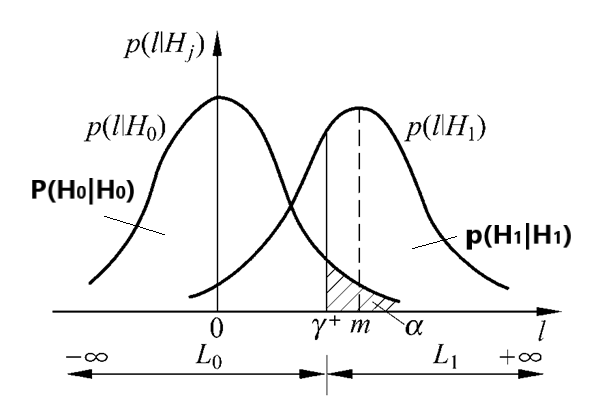
\includegraphics[scale=0.2]{mgt0}\\
	\scriptsize
	\textcolor{blue}{$p(l|H_j)(j=0,1)$: 假设$H_j$下观测信号的概率密度函数; $r^+=\frac{\sigma^2\ln\eta}{Nm}+\frac{m}{2}; \alpha=P(H_1|H_0)$}
\end{columns}
\end{frame}

\begin{frame}[shrink]
\begin{columns}
	\column{0.4\textwidth}
	观测信号$(\bm{x}=\{x_1,x_2,\dots,x_N\})$
	\begin{align*}
	&(\bm{x}|H_0)\sim\mathcal{N}(0,\sigma^2), &(\bm{x}|H_1)\sim\mathcal{N}(A,\sigma^2)
	\end{align*}
	检验统计量$l(x)$:
	\begin{align*}
	&(l|H_0)\sim\mathcal{N}(0,\frac{1}{N}\sigma^2), &(l|H_1)\sim\mathcal{N}(A,\frac{1}{N}\sigma^2)
	\end{align*}
	归一化后, $(l|H_j)\sim\mathcal{N}(0,1)$
	\column{0.4\textwidth}
	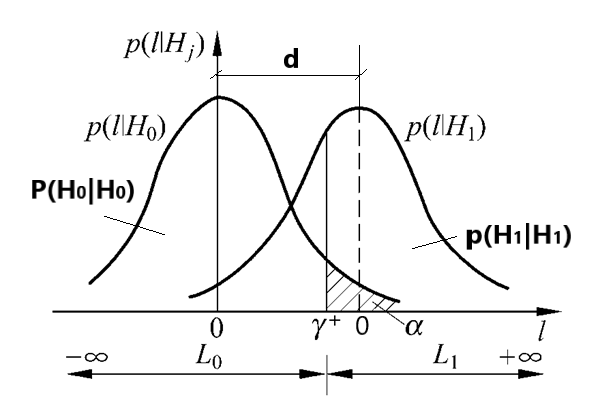
\includegraphics[scale=0.2]{0A}\\
	\scriptsize
	\textcolor{blue}{$p(l|H_j)(j=0,1)$: 假设$H_j$下观测信号的概率密度函数; $r^+=\frac{\ln\eta}{d}+\frac{d}{2}; \alpha=P(H_1|H_0)$}
\end{columns}

\bigskip

判决表达式:
\[
l(x)\mathop{=}^{def}\frac{1}{N}\sum\limits_{i=1}^Nx_i\mathop{\gtrless}_{H_0}^{H_1}\frac{\sigma^2\ln\eta}{NA}+\frac{A}{2}\mathop{=}^{def}\gamma^+
\]

判决概率:(其中,信噪比$d^2=\frac{NA^2}{\sigma^2}$)
\begin{align*}
	P(H_1|H_0)&=Q\left(\frac{\ln\eta}{d}+\frac{d}{2}\right), &P(H_0|H_0)&=1-Q\left(\frac{\ln\eta}{d}+\frac{d}{2}\right)\\
	P(H_1|H_1)&=Q\left(\frac{\ln\eta}{d}-\frac{d}{2}\right),
	&P(H_0|H_1)&=1-Q\left(\frac{\ln\eta}{d}-\frac{d}{2}\right)
\end{align*}
\end{frame}

\begin{frame}{贝叶斯检测性能分析小结(ex3小结2)}
\begin{columns}
	\column{0.4\textwidth}
	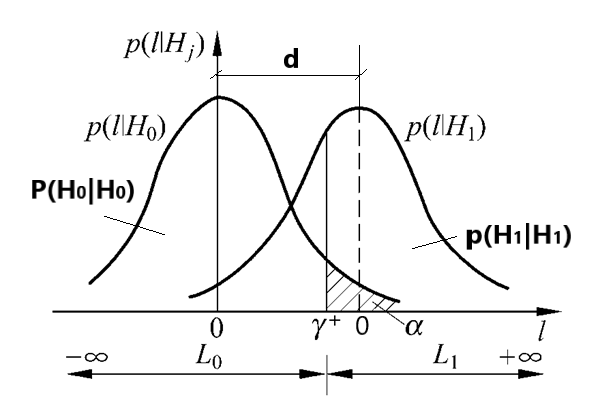
\includegraphics[scale=0.2]{0A}
	\scriptsize
	\textcolor{blue}{$p(l|H_j)(j=0,1)$: 假设$H_j$下观测信号的概率密度函数; $r^+=\frac{\ln\eta}{d}+\frac{d}{2}; \alpha=P(H_1|H_0)$}
	\column{0.4\textwidth}
	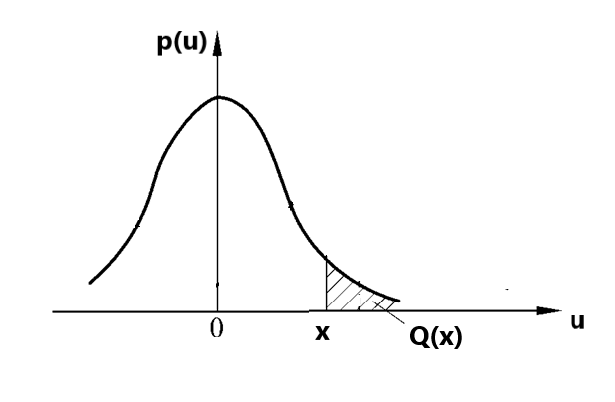
\includegraphics[scale=0.2]{Qx}
	\scriptsize
	\textcolor{red}{$Q(x)=\int_{x}^{\infty}\frac{1}{\sqrt{2\pi}}\exp(-\frac{u^2}{2})du$.}\\
	\textcolor{red}{$Q(x)$是单调递减函数, 其反函数: $Q^{-1}[\bullet]$}
\end{columns}

\bigskip

 因为$P(H_1|H_0)=Q(\ln\eta/d+d/2) \implies \ln\eta/d=Q^{-1}[P(H_1|H_0)]-d/2$\\
这样有:
\begin{align*}
P(H_1|H_1)&=Q\left(\ln\eta/d-d/2\right)\\
&=Q[Q^{-1}[P(H_1|H_0)]-d/2-d/2]=Q[Q^{-1}[P(H_1|H_0)]-d]
\end{align*}
\colorbox{yellow}{这说明, 当给定$P(H_1|H_0)$时, $P(H_1|H_1)$随功率信噪比$(d^2=NA^2/\sigma^2)$单调增加。} 
\colorbox{green}{另一方面, 采样次数$N\uparrow\implies d\uparrow$, $p(l|H_0),p(l|H_1)$的间距$d\uparrow$,  检测性能$\uparrow$。} 
\end{frame}

\begin{frame}[shrink]
\frametitle{ex3小结(1)}
\begin{columns}
	\column{0.4\textwidth}
	$N$次独立采样, 样本为$x_i(i=1,2,\dots,N)$
	\begin{align*}
	&&n_i\sim\mathcal{N}(0,\sigma^2)\\ 
	H_0 &:x_i=n_i   &(l|H_0)\sim\mathcal{N}(0,\frac{\sigma^2}{N})\\
	H_1 &:x_i=A+n_i &(l|H_1)\sim\mathcal{N}(m,\frac{\sigma^2}{N})
	\end{align*}
	\column{0.4\textwidth}
	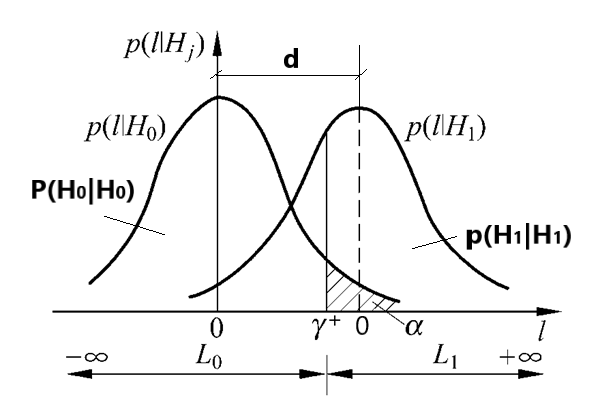
\includegraphics[scale=0.2]{0A}\\
	\scriptsize
	\textcolor{blue}{$p(l|H_j)(j=0,1)$: 假设$H_j$下观测信号的概率密度函数; $r^+=\frac{\ln\eta}{d}+\frac{d}{2}; \alpha=P(H_1|H_0)$}
\end{columns}

\bigskip

检验统计量$l(x)$:
\begin{align*}
&(l|H_0)\sim\mathcal{N}(0,\frac{1}{N}\sigma^2), &(l|H_1)\sim\mathcal{N}(A,\frac{1}{N}\sigma^2)
\end{align*}
归一化后, $(l|H_j)\sim\mathcal{N}(0,1)$

判决表达式:
\[
l(x)\mathop{=}^{def}\frac{1}{N}\sum\limits_{i=1}^Nx_i\mathop{\gtrless}_{H_0}^{H_1}\frac{\sigma^2\ln\eta}{NA}+\frac{A}{2}\mathop{=}^{def}\gamma^+
\]

判决概率:(其中,信噪比$d^2=\frac{NA^2}{\sigma^2}$)
\begin{align*}
P(H_1|H_0)&=Q\left(\frac{\ln\eta}{d}+\frac{d}{2}\right), &P(H_0|H_0)&=1-Q\left(\frac{\ln\eta}{d}+\frac{d}{2}\right)\\
P(H_1|H_1)&=Q\left(\frac{\ln\eta}{d}-\frac{d}{2}\right),
&P(H_0|H_1)&=1-Q\left(\frac{\ln\eta}{d}-\frac{d}{2}\right)
\end{align*}
\end{frame}

\begin{frame}[shrink]
\frametitle{ex3---观测量$(l|H_0)$}
\textcolor{blue}{\textbf{性能分析:}}
\[
\frac{1}{N}\sum\limits_{i=1}^{N}x_i\mathop{\gtrless}\limits_{H_0}^{H_1}\frac{\sigma^2\ln\eta}{NA}+\frac{A}{2}\mathop{=}\limits^{def}\gamma
\]
\textbf{统计量  }\qquad $l(x)\mathop{=}\limits^{def}\frac{1}{N}\sum\limits_{i=1}^{N}x_i$\\
\textbf{假设$H_0$条件下, 统计量$l(x)$为高斯分布, 均值和方差分别为}
\begin{align*}
E[l|H_0]&=E\left[\frac{1}{N}\sum\limits_{i=1}^{N}(x_i|H_0)\right]=E\left[\frac{1}{N}\sum\limits_{i=1}^{N}n_i\right]=\frac{1}{N}\sum\limits_{i=1}^{N}E[n_i]=0\\
Var[l|H_0]&=E\left[(l|H_0-E(l|H_0))^2\right]=E\left[\left(\frac{1}{N}\sum\limits_{i=1}^{N}n_i\right)^2\right]\\
&=\frac{1}{N^2}\sum\limits_{i=1}^{N}E[n_i^2]=\frac{1}{N^2}\sum\limits_{i=1}^{N}\sigma^2=\frac{\sigma^2}{N}\\
\textbf{因此, }(l|H_0)\sim\mathcal{N}(0,\frac{\sigma^2}{N})\\
p(l|H_0)&=\frac{1}{\sqrt{2\pi Var[l|H_0]}}\exp\left[-\frac{(l-E[l|H_0])^2}{2 Var[l|H_0]}\right]=\frac{\sqrt{N}}{\sqrt{2\pi\sigma^2}}\exp\left[-\frac{Nl^2}{2\sigma^2}\right]
\end{align*}
\end{frame}

\begin{frame}[shrink]
\frametitle{ex3---观测量$(l|H_1)$}
\textcolor{blue}{\textbf{性能分析:}}
\[
\frac{1}{N}\sum\limits_{i=1}^{N}x_i\mathop{\gtrless}\limits_{H_0}^{H_1}\frac{\sigma^2\ln\eta}{NA}+\frac{A}{2}\mathop{=}\limits^{def}\gamma
\]
\textbf{统计量  }\qquad $l(x)\mathop{=}\limits^{def}\frac{1}{N}\sum\limits_{i=1}^{N}x_i$\\
\textbf{假设$H_1$条件下, 统计量$l(x)$为高斯分布, 均值和方差分别为}
\begin{align*}
E[l|H_1]&=E\left[\frac{1}{N}\sum\limits_{i=1}^{N}(x_i|H_1)\right]=E\left[\frac{1}{N}\sum\limits_{i=1}^{N}(A+n_i)\right]=A+\frac{1}{N}\sum\limits_{i=1}^{N}E[n_i]=A\\
Var[l|H_1]&=E\left[(l|H_1-E(l|H_1))^2\right]=E\left[\left(\frac{1}{N}\sum\limits_{i=1}^{N}(A+n_i)-A\right)^2\right]\\
&=\frac{1}{N^2}\sum\limits_{i=1}^{N}E[n_i^2]=\frac{1}{N^2}\sum\limits_{i=1}^{N}\sigma^2=\frac{\sigma^2}{N}\\
\textbf{因此, }(l|H_1)\sim\mathcal{N}(A,\frac{\sigma^2}{N})\\
p(l|H_1)&=\frac{1}{\sqrt{2\pi Var[l|H_1]}}\exp\left[-\frac{(l-E[l|H_1])^2}{2 Var[l|H_1]}\right]=\frac{\sqrt{N}}{\sqrt{2\pi\sigma^2}}\exp\left[-\frac{N(l-A)^2}{2\sigma^2}\right]
\end{align*}
\end{frame}

\begin{frame}[shrink]
\frametitle{ex4---$l|H_0$}
\begin{columns}
	\column{0.4\textwidth}
	\textcolor{blue}{\textbf{$N$次独立采样,样本为:}}
	\begin{align*}
	&H_0: x_i=1+n_i, i=1,2,\dots,N\\
	&H_1: x_i=-1+n_i, i=1,2,\dots,N
	\end{align*}
	\column{0.4\textwidth}
	\textcolor{blue}{\textbf{计算平均代价:}}
	\[
	\frac{1}{N}\sum\limits_{i=1}^{N}x_i\mathop{\gtrless}\limits_{H_0}^{H_1}\frac{\sigma^2\ln\eta}{2N}=-\frac{\ln 3}{4N}\mathop{=}\limits^{def}\gamma
	\]
	\textbf{统计量  }\qquad $l(x)\mathop{=}\limits^{def}\frac{1}{N}\sum\limits_{i=1}^{N}x_i$\\
\end{columns}
\textbf{假设$H_0$条件下, 统计量$l(x)$为高斯分布, 均值和方差分别为}
\begin{align*}
E[l|H_0]&=E\left[\frac{1}{N}\sum\limits_{i=1}^{N}(x_i|H_0)\right]=E\left[\frac{1}{N}\sum\limits_{i=1}^{N}(1+n_i)\right]\\
&=\frac{1}{N}\sum\limits_{i=1}^{N}E[(1+n_i)]=\frac{1}{N}\sum\limits_{i=1}^{N}[E(1)+E(n_i)]=\frac{1}{N}\sum\limits_{i=1}^{N}[1+0]=1\\
Var[l|H_0]&=E\left[(l|H_0-E[l|H_0]))^2\right]=E\left[\left(\frac{1}{N}\sum\limits_{i=1}^{N}(1+n_i)-E(l)\right)^2\right]\\
&=E\left[\left(\frac{1}{N}\sum\limits_{i=1}^{N}(1+n_i)-1\right)^2\right]=E\left[\left(\frac{1}{N}\sum\limits_{i=1}^{N}n_i\right)^2\right]\\
&=\frac{1}{N^2}\sum\limits_{i=1}^{N}E[n_i^2]=\frac{1}{N^2}\sum\limits_{i=1}^{N}\sigma^2=\frac{\sigma^2}{N}\\
\textbf{因此, }(l|H_0)\sim\mathcal{N}(1,\frac{\sigma^2}{N})\\
p(l|H_0)&=\frac{1}{\sqrt{2\pi Var[l|H_0]}}\exp\left[-\frac{(l-E[l|H_0])^2}{2 Var[l|H_0]}\right]=\frac{\sqrt{N}}{\sqrt{2\pi\sigma^2}}\exp\left[-\frac{N(l-1)^2}{2\sigma^2}\right]
\end{align*}
\end{frame}

\begin{frame}[shrink]
\frametitle{ex4---$l|H_1$}
\begin{columns}
	\column{0.4\textwidth}
	\textcolor{blue}{\textbf{$N$次独立采样,样本为:}}
	\begin{align*}
	&H_0: x_i=1+n_i, i=1,2,\dots,N\\
	&H_1: x_i=-1+n_i, i=1,2,\dots,N
	\end{align*}
	\column{0.4\textwidth}
	\textcolor{blue}{\textbf{计算平均代价:}}
	\[
	\frac{1}{N}\sum\limits_{i=1}^{N}x_i\mathop{\gtrless}\limits_{H_0}^{H_1}\frac{\sigma^2\ln\eta}{2N}=-\frac{\ln 3}{4N}\mathop{=}\limits^{def}\gamma
	\]
	\textbf{统计量  }\qquad $l(x)\mathop{=}\limits^{def}\frac{1}{N}\sum\limits_{i=1}^{N}x_i$\\
\end{columns}
\textbf{假设$H_1$条件下, 统计量$l(x)$为高斯分布, 均值和方差分别为}
\begin{align*}
E[l|H_1]&=E\left[\frac{1}{N}\sum\limits_{i=1}^{N}(x_i|H_1)\right]=E\left[\frac{1}{N}\sum\limits_{i=1}^{N}(-1+n_i)\right]\\
&=\frac{1}{N}\sum\limits_{i=1}^{N}E[(1+n_i)]=\frac{1}{N}\sum\limits_{i=1}^{N}[E(-1)+E(n_i)]=\frac{1}{N}\sum\limits_{i=1}^{N}[-1+0]=-1\\
Var[l|H_1]&=E\left[(l|H_1-E[l|H_1]))^2\right]=E\left[\left(\frac{1}{N}\sum\limits_{i=1}^{N}(-1+n_i)-E(l)\right)^2\right]\\
&=E\left[\left(\frac{1}{N}\sum\limits_{i=1}^{N}(-1+n_i)+1\right)^2\right]=E\left[\left(\frac{1}{N}\sum\limits_{i=1}^{N}n_i\right)^2\right]\\
&=\frac{1}{N^2}\sum\limits_{i=1}^{N}E[n_i^2]=\frac{1}{N^2}\sum\limits_{i=1}^{N}\sigma^2=\frac{\sigma^2}{N}\\
\textbf{因此, }(l|H_1)\sim\mathcal{N}(-1,\frac{\sigma^2}{N})\\
p(l|H_1)&=\frac{1}{\sqrt{2\pi Var[l|H_1]}}\exp\left[-\frac{(l-E[l|H_1])^2}{2 Var[l|H_1]}\right]=\frac{\sqrt{N}}{\sqrt{2\pi\sigma^2}}\exp\left[-\frac{N(l+1)^2}{2\sigma^2}\right]
\end{align*}
\end{frame}

\begin{frame}[shrink]
\frametitle{公式推导练习(1)}
检验统计量:
\[l(x)=\frac{1}{N}\sum\limits_{i=1}^{N}(a+bn_i), i=1,2,\dots,N\]
其中: $n_i\sim\mathcal{N}(0,\sigma_n^2)$, 即$E[n_i]=0,Var[n_i]=E\left[(n_i-E[n_i])^2\right]=E[n_i^2]=\sigma_n^2$\\
\textbf{统计量$l(x)$是高斯随机变量$n_i$的线性组合, 服从高斯分布, 均值和方差分别为}
\begin{align*}
E[l]&=E\left[\frac{1}{N}\sum\limits_{i=1}^{N}(a+bn_i)\right]=\frac{1}{N}\sum\limits_{i=1}^{N}E[a+bn_i]\\
&=a+\frac{b}{N}\sum\limits_{i=1}^{N}E[n_i]=a &&\text{by } E[n_i]=0\\
Var[l]&=E[(l-E(l))^2]=E\left[\left(\frac{1}{N}\sum\limits_{i=1}^{N}(a+bn_i)-a\right)^2\right]\\
&=E\left[\left(\frac{1}{N}\sum\limits_{i=1}^{N}(bn_i)\right)^2\right]=E\left[\left(\frac{b}{N}\sum\limits_{i=1}^{N}n_i\right)^2\right]\\
&=\left(\frac{b}{N}\right)^2\sum\limits_{i=1}^{N}E[n_i^2]=\left(\frac{b}{N}\right)^2N\sigma_n^2=\frac{b^2\sigma_n^2}{N} &&\text{by } E[n_i^2]=\sigma_n^2\\
\end{align*}
\end{frame}

\begin{frame}[shrink]
\frametitle{公式推导练习(2)}
检验统计量:
\[l(x)=\frac{1}{N}\sum\limits_{i=1}^{N}(m+n_i),i=1,2,\dots,N\]
其中: $m$是常数, $n_i\sim\mathcal{N}(0,\sigma_n^2)$, 即$E[n_i]=0,Var[n_i]=E\left[(n_i-E[n_i])^2\right]=E[n_i^2]=\sigma_n^2$\\
\textbf{统计量$l(x)$是高斯随机变量$n_i$的线性组合, 服从高斯分布, 均值和方差分别为}
\begin{align*}
E[l]&=E\left[\frac{1}{N}\sum\limits_{i=1}^{N}(m+n_i)\right]=\frac{1}{N}\sum\limits_{i=1}^{N}E[m+n_i]\\
&=m+\frac{1}{N}\sum\limits_{i=1}^{N}E[n_i] &&\text{by } E[n_i]=0\\
&=m\\
Var[l]&=E[(l-E(l))^2]=E\left[\left(\frac{1}{N}\sum\limits_{i=1}^{N}(m+n_i)-m\right)^2\right]\\
&=E\left[\left(\frac{1}{N}\sum\limits_{i=1}^{N}n_i\right)^2\right]=E\left[\left(\frac{1}{N}\sum\limits_{i=1}^{N}n_i\right)^2\right]\\
&=\frac{1}{N^2}\sum\limits_{i=1}^{N}E[n_i^2]=\frac{1}{N^2}N\sigma_n^2 &&\text{by } E[n_i^2]=\sigma_n^2\\
&=\frac{\sigma_n^2}{N}
\end{align*}
\end{frame}

\begin{frame}[shrink]
\frametitle{ex5推导(1)}
两个假设下,观测量$x$均服从高斯分布,$(x|H_0)\sim\mathcal{N}(0, \sigma^2), (x|H_1)\sim\mathcal{N}(A, \sigma^2)$.
\begin{align*}
p(x|H_0)&=\left(\frac{1}{2\pi\sigma^2}\right)^{1/2}\exp\left(-\frac{x^2}{2\sigma^2}\right)\\
p(x|H_1)&=\left(\frac{1}{2\pi\sigma^2}\right)^{1/2}\exp\left[-\frac{(x-A)^2}{2\sigma^2}\right]
\end{align*}
两个假设先验概率等概,且$c_{00}=c_{11}=0,c_{10}=c_{01}=1$, 所以似然比检验判别式为:
\[\lambda(x)=\frac{p(x|H_1)}{p(x|H_0)}=\exp\left(\frac{2Ax-A^2}{2\sigma^2}\right)\mathop{\gtrless}_{H_0}^{H_1}\eta=1 \]
化简得判决表达式:
\[x\mathop{\gtrless}_{H_0}^{H_1}\frac{A}{2} \]
由于检验统计量$l(x)=x$,所以
\begin{align*}
p(l|H_0)&=\left(\frac{1}{2\pi\sigma^2}\right)^{1/2}\exp\left(-\frac{l^2}{2\sigma^2}\right)\\
p(l|H_1)&=\left(\frac{1}{2\pi\sigma^2}\right)^{1/2}\exp\left[-\frac{(l-A)^2}{2\sigma^2}\right]
\end{align*}
\end{frame}

\begin{frame}[shrink]
\frametitle{ex5推导(2)}
又因为检测判决门限$\gamma=\frac{A}{2}$, 所以两种错误判决概率分别为
\begin{align*}
P(H_1|H_0)&=\int_{\gamma}^{\infty}p(l|H_0)dl=\int_{\frac{A}{2}}^{\infty}\left(\frac{1}{2\pi\sigma^2}\right)^{1/2}\exp\left(-\frac{l^2}{2\sigma^2}\right)dl\\
&\mathop{=}^{l=\sigma u}\int_{\frac{A}{2\sigma}}^{\infty}\left(\frac{1}{2\pi}\right)^{1/2}\exp\left(-\frac{u^2}{2}\right)du\\
&=Q[\frac{A}{2\sigma}]=Q[\frac{d}{2}] \qquad \text{ by } d^2\mathop{=}^{def}A^2/\sigma^2
\end{align*}
\begin{columns}
	\column{0.4\textwidth}
	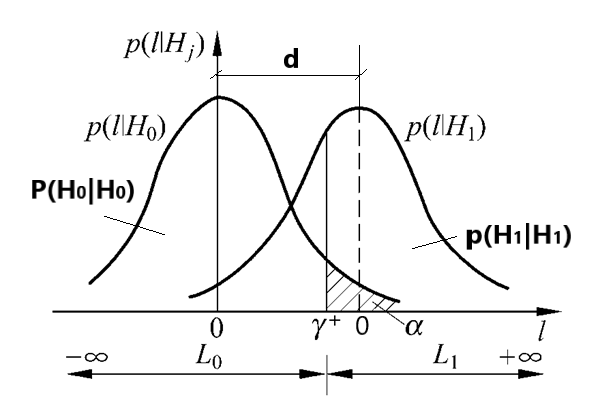
\includegraphics[scale=0.2]{0A}
	\scriptsize
	\textcolor{blue}{$p(l|H_j)(j=0,1)$: 假设$H_j$下观测信号的概率密度函数; $\alpha=P(H_1|H_0)$}
	\column{0.4\textwidth}
	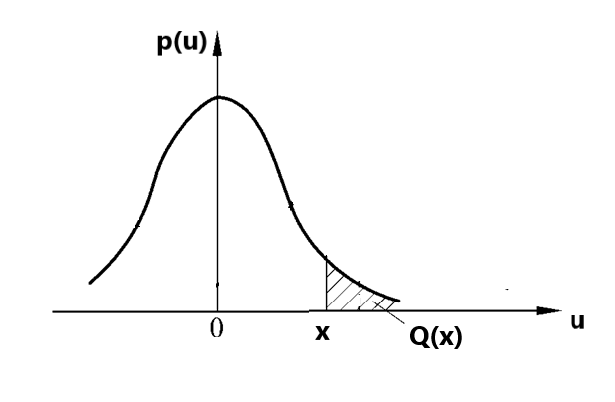
\includegraphics[scale=0.2]{Qx}
	\scriptsize
	\textcolor{red}{$Q(x)=\int_{x}^{\infty}\frac{1}{\sqrt{2\pi}}\exp(-\frac{u^2}{2})du$.}\\
	\textcolor{red}{$Q(x)$是单调递减函数, 其反函数: $Q^{-1}[\bullet]$}
\end{columns}
\end{frame}

\begin{frame}[shrink]
\frametitle{ex5推导(3)}
\begin{align*}
P(H_0|H_1)&=\int_{-\infty}^{\gamma}p(l|H_1)dl=\int_{-\infty}^{\frac{A}{2}}\left(\frac{1}{2\pi\sigma^2}\right)^{1/2}\exp\left(-\frac{(l-A)^2}{2\sigma^2}\right)dl\\
&\mathop{=}^{l=A+\sigma u}\int_{-\infty}^{-\frac{A}{2\sigma}}\left(\frac{1}{2\pi}\right)^{1/2}\exp\left(-\frac{u^2}{2}\right)du\\
&=1-\int_{-\frac{A}{2\sigma}}^{\infty}\left(\frac{1}{2\pi}\right)^{1/2}\exp\left(-\frac{u^2}{2}\right)du\\
&=1-Q[-\frac{A}{2\sigma}]=1-Q[-\frac{d}{2}]=Q[\frac{d}{2}]\qquad \text{ by } d^2\mathop{=}^{def}A^2/\sigma^2
\end{align*}
\begin{columns}
	\column{0.4\textwidth}
	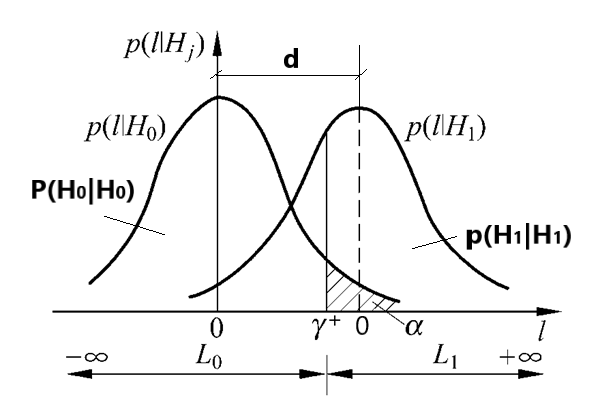
\includegraphics[scale=0.2]{0A}
	\scriptsize
	\textcolor{blue}{$p(l|H_j)(j=0,1)$: 假设$H_j$下观测信号的概率密度函数; $\alpha=P(H_1|H_0)$}
	\column{0.4\textwidth}
	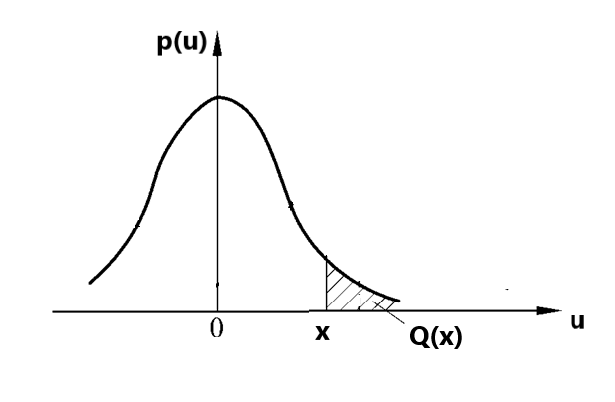
\includegraphics[scale=0.2]{Qx}
	\scriptsize
	\textcolor{red}{$Q(x)=\int_{x}^{\infty}\frac{1}{\sqrt{2\pi}}\exp(-\frac{u^2}{2})du$.}\\
	\textcolor{red}{$Q(x)$是单调递减函数, 其反函数: $Q^{-1}[\bullet]$}
\end{columns}
\end{frame}

\begin{frame}[shrink]
\frametitle{ex5推导(4)}
两种错误判决概率:
\begin{align*}
P(H_1|H_0)=Q[\frac{d}{2}],\qquad P(H_0|H_1)=Q[\frac{d}{2}]
\end{align*}
其中, $d^2\mathop{=}\limits^{def}A^2/\sigma^2$。所以, 平均错误概率$P_e$为
\begin{align*}
P_e&=P(H_0)P(H_1|H_0)+P(H_1)P(H_0|H_1)\\
&=\frac{1}{2}Q[\frac{d}{2}]+\frac{1}{2}Q[\frac{d}{2}]=Q[\frac{d}{2}]
\end{align*}
\colorbox{yellow}{$Q(x)$是单调递减函数,信噪比$d$越高, 平均错误概率越小,检测性能越好。}
\begin{columns}
	\column{0.4\textwidth}
	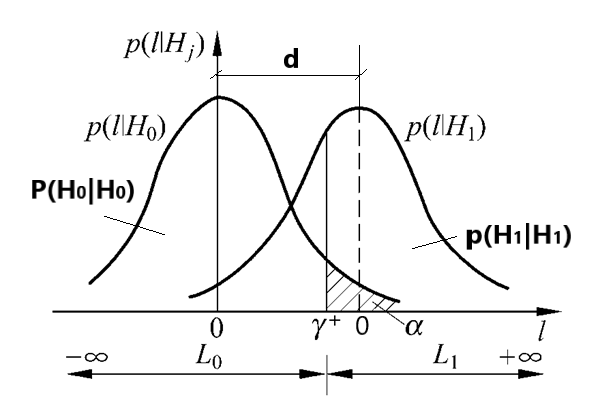
\includegraphics[scale=0.2]{0A}
	\scriptsize
	\textcolor{blue}{$p(l|H_j)(j=0,1)$: 假设$H_j$下观测信号的概率密度函数; $\alpha=P(H_1|H_0)$}
	\column{0.4\textwidth}
	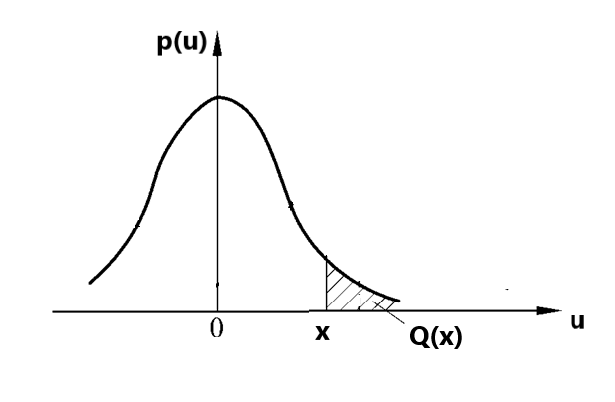
\includegraphics[scale=0.2]{Qx}
	\scriptsize
	\textcolor{red}{$Q(x)=\int_{x}^{\infty}\frac{1}{\sqrt{2\pi}}\exp(-\frac{u^2}{2})du$.}\\
	\textcolor{red}{$Q(x)$是单调递减函数, 其反函数: $Q^{-1}[\bullet]$}
\end{columns}
\end{frame}

\begin{frame}[shrink]
\frametitle{最大后验概率准则}
在贝叶斯准则中, 当代价因子满足: $c_{10}-c_{00}=c_{01}-c_{11}$时 
\[\lambda(\bm{x})=\frac{p(\bm{x}|H_1)}{p(\bm{x}|H_0)}\mathop{\gtrless}\limits_{H_0}^{H_1}\frac{P(H_0)}{P(H_1)}\implies P(H_1)p(\bm{x}|H_1)\mathop{\gtrless}\limits_{H_0}^{H_1}P(H_0)p(\bm{x}|H_0)\]
由条件概率公式,有
\[P(H_1|(\bm{x}\le X\le \bm{x}+d\bm{x}))=\frac{P((\bm{x}\le X\le \bm{x}+d\bm{x})|H_1)P(H_1)}{P(\bm{x}\le X\le \bm{x}+d\bm{x})}\]
当$d\bm{x}$很小时,有$P((\bm{x}\le X\le \bm{x}+d\bm{x})|H_1)=p(\bm{x}|H_1)d\bm{x},\quad P(\bm{x}\le X\le \bm{x}+d\bm{x})=p(\bm{x})d\bm{x}$\\
$P(H_1|(\bm{x}\le X\le \bm{x}+d\bm{x}))=P(H_1|\bm{x})$, 从而得
\[P(H_1|\bm{x})=\frac{p(\bm{x}|H_1)d\bm{x}P(H_1)}{p(\bm{x})d\bm{x}}=\frac{p(\bm{x}|H_1)P(H_1)}{p(\bm{x})}\]
\[\implies P(H_1)p(\bm{x}|H_1)=p(\bm{x})P(H_1|\bm{x}) \]
类似地,可得
\[P(H_0)p(\bm{x}|H_0)=p(\bm{x})P(H_0|\bm{x}) \]
\end{frame}

\begin{frame}[shrink]
\frametitle{最大后验概率准则}
\[P(H_1)p(\bm{x}|H_1)=p(\bm{x})P(H_1|\bm{x}),\quad P(H_0)p(\bm{x}|H_0)=p(\bm{x})P(H_0|\bm{x}) \]
\[\lambda(\bm{x})=\frac{p(\bm{x}|H_1)}{p(\bm{x}|H_0)}\mathop{\gtrless}\limits_{H_0}^{H_1}\frac{P(H_0)}{P(H_1)}\implies P(H_1)p(\bm{x}|H_1)\mathop{\gtrless}\limits_{H_0}^{H_1}P(H_0)p(\bm{x}|H_0)\]
\[p(\bm{x})P(H_1|\bm{x})\mathop{\gtrless}\limits_{H_0}^{H_1}p(\bm{x})P(H_0|\bm{x}) \]
\[P(H_1|\bm{x})\mathop{\gtrless}\limits_{H_0}^{H_1}P(H_0|\bm{x}) \]
$P(H_j|\bm{x})(j=0,1)$表示已经获得观测量$\bm{x}$的条件下,假设$H_j$为真时的概率, 称为\textbf{后验概率}。\\
按照最小平均代价的贝叶斯准则在代价因子满足: $c_{10}-c_{00}=c_{01}-c_{11}$时,就成为\textbf{最大后验概率准则(maximum a posteriori probability criterion)} 
\end{frame}

\begin{frame}{术语}
\begin{itemize}
	\item $H_1: A+n$代表雷达检测有回波信号, $H_0: x=n$仅含噪声信号。
	\item 虚警概率$P_F\mathop{=}\limits^{def}P(H_1|H_0)$: False alarm, 假设$H_0$为真的条件下,判决$H_1$成立的概率。是个假判决。
	\item 漏警概率$P_M\mathop{=}\limits^{def}P(H_0|H_1)$: Miss alarm, 假设$H_1$为真的条件下, 判决$H_0$成立的概率。是个遗漏的判决。
	\item 漏警概率$P_D\mathop{=}\limits^{def}P(H_1|H_1)$: Ditection alarm, 假设$H_1$为真的条件下, 判决$H_1$成立的概率。是个正确检测的判决。
\end{itemize}
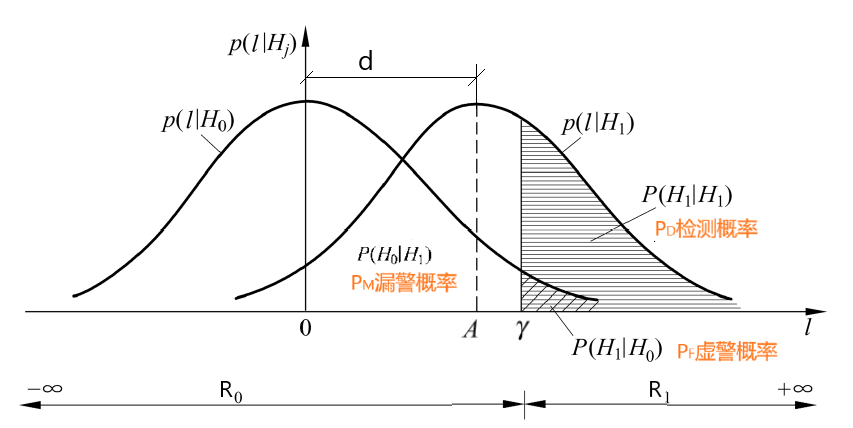
\includegraphics[scale=0.25]{R0R1}
\end{frame}

\begin{frame}{平均代价}
假设$H_j$为真,判决所付出的平均代价为:
\[C(H_j)=\sum\limits_{i=0}^{1}c_{ij}P(H_i|H_j) \]
\begin{align*}
&\text{判决$H_0$成立的代价} &C(H_0)=c_{00}P(H_0|H_0)+c_{10}P(H_1|H_0)\\
&\text{判决$H_1$成立的代价} &C(H_1)=c_{01}P(H_0|H_1)+c_{11}P(H_1|H_1)\\
&\text{总代价:} &C=P(H_0)C(H_0)+P(H_1)C(H_1)
\end{align*}
\end{frame}

\begin{frame}[shrink]
\frametitle{平均代价$C(P_1)$是先验概率$P_1$的严格上凸函数}
\begin{columns}%0.6 0.4表示相对比例
	\column{0.5\textwidth}
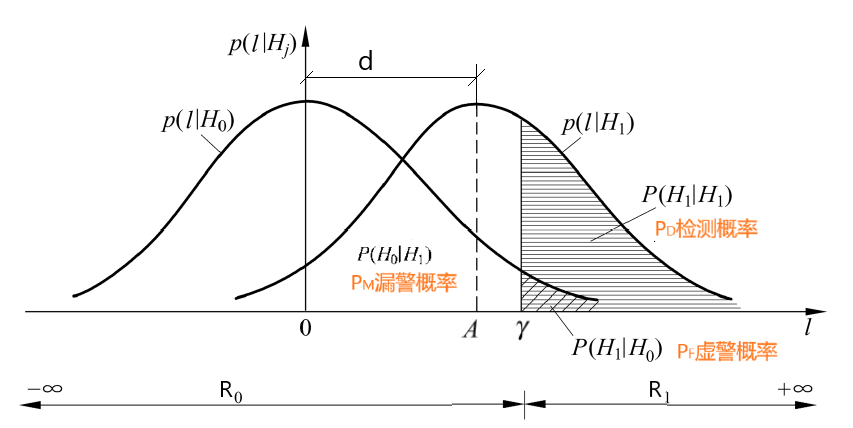
\includegraphics[scale=0.25]{R0R1}
	\column{0.3\textwidth}
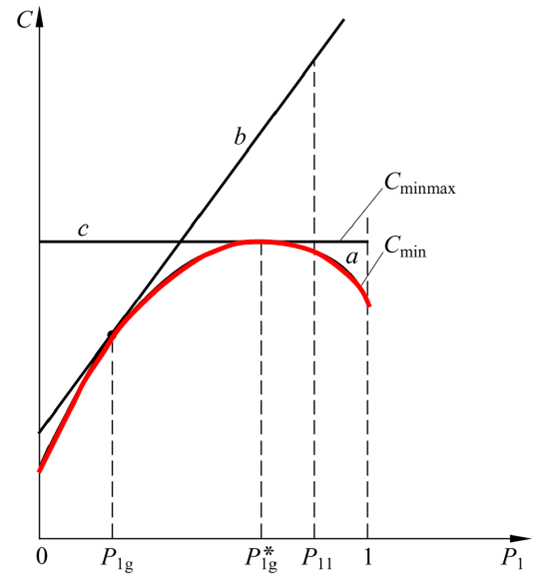
\includegraphics[scale=0.25]{C-P1}
\end{columns}
\begin{align*}
&\eta\mathop{=}^{def}\eta(P_1)=\frac{P(H_0)(c_{10}-c_{00})}{P(H_1)(c_{01}-c_{11})}=\frac{(1-P_1)(c_{10}-c_{00})}{P_1(c_{01}-c_{11})}=\frac{1}{P_1(c_{01}-c_{11})}-\frac{c_{10}-c_{00}}{c_{01}-c_{11}}\\
&\text{先验概率}P_1\mathop{=}^{def}P(H_1),\quad P_F\mathop{=}^{def}P_F(P_1)=P(H_1|H_0),\quad  P_M\mathop{=}^{def}P_M(P_1)=P(H_0|H_1)\\
&P(H_0|H_0)=1-P(H_1|H_0)=1-P_F(P_1),\quad P(H_1|H_1)=1-P(H_0|H_1)=1-P_M(P_1)\\
&C(P_1)=c_{00}+(c_{10}-c_{00})P_F(P_1)+  \quad \textbf{平均代价$C(P_1)$是先验概率$P_1$的严格上凸函数}\\
&P_1[(c_{11}-c_{00})+(c_{01}-c_{11})P_M(P_1)-(c_{10}-c_{00})P_F(P_1)]
\end{align*}
$P_1\uparrow\implies \eta\downarrow, P_M\downarrow, P_F\uparrow, P_D\uparrow, C\uparrow\sim C_{minmax}\sim\downarrow$
\end{frame}

\begin{frame}[shrink]
\frametitle{直线$C(P_1,P_{1g})$与上凸函数$C(P_1)$}
\textbf{目的: 尽可能避免产生过分大的代价,使极大可能代价最小化。}
\begin{enumerate}
	\item 猜测一个先验概率$P_{1g}$, 以$\eta(P_{1g})$为门限进行判决。
	\item $P_{1g}$确定, $P_M(P_{1g})$和$P_F(P_{1g})$即可确定。
	\item $P_{1g}$确定,则$C(P_1,P_{1g})$表示与上凸函数曲线$C(P_1)$的切线,如图中的直线$b$, $c$。
\end{enumerate}
\begin{columns}
	\column{0.5\textwidth}
	\begin{align*}
	&\eta=\eta(P_{1g})=\frac{1}{P_{1g}(c_{01}-c_{11})}-\frac{c_{10}-c_{00}}{c_{01}-c_{11}}\\
	&C(P_1)=c_{00}+(c_{10}-c_{00})P_F(P_1)+\\
	&P_1[(c_{11}-c_{00})+(c_{01}-c_{11})P_M(P_1)-(c_{10}-c_{00})P_F(P_1)]\\
	&C(P_1,P_{1g})=c_{00}+(c_{10}-c_{00})P_F(P_{1g})+\\
	&P_1[(c_{11}-c_{00})+(c_{01}-c_{11})P_M(P_{1g})-(c_{10}-c_{00})P_F(P_{1g})]
	\end{align*}
	\column{0.3\textwidth}
	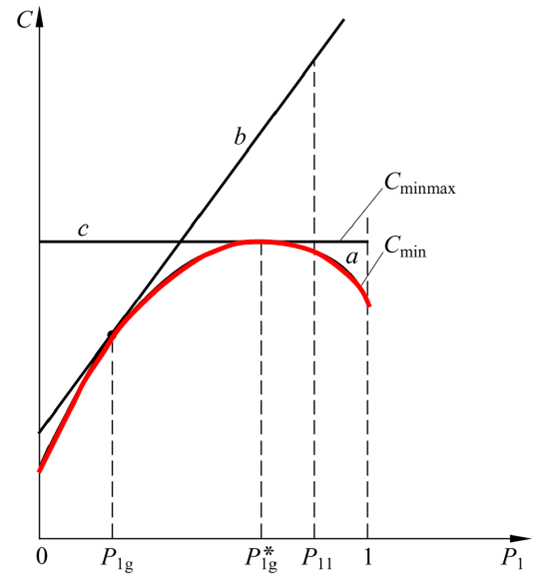
\includegraphics[scale=0.25]{C-P1}
\end{columns}
\end{frame}

\begin{frame}[shrink]
\frametitle{极小极大化准则}
\textbf{目的: 尽可能避免产生过分大的代价,使极大可能代价最小化。}
\begin{enumerate}
	\setcounter{enumi}{3}
	\item 如果实际$P_1=P_{1g}$, 平均代价最小, 在直线$b$与$C(P_1)$的切点处, $C(P_1=P_{1g},P(_{1g}))$。
	\item 如果实际$P_1\ne P_{1g}$, 比如$P_1=P_{11}$, 则平均代价远大于$C(P_1=P_{1g},P(_{1g}))$, 在直线$P_1=P_{11}$与直线$b$的交点处。
	\item 如果猜测的先验概率为$P_{1g}^{\ast}$,则无论实际的先验概率$P_1$为多大,平均代价都等于$C_{minmax}$, 而不会产生过分大的代价。\textbf{产生的代价与先验概率$P_1$无关。$P_{1g}^{\ast}$即是先验概率$P_1$最理想的猜测值。}
\end{enumerate}
\begin{columns}
	\column{0.5\textwidth}
	\begin{align*}
	&C(P_1,P_{1g})=c_{00}+(c_{10}-c_{00})P_F(P_{1g})+\\
	&P_1[(c_{11}-c_{00})+(c_{01}-c_{11})P_M(P_{1g})-(c_{10}-c_{00})P_F(P_{1g})]
	\end{align*}
	\column{0.3\textwidth}
	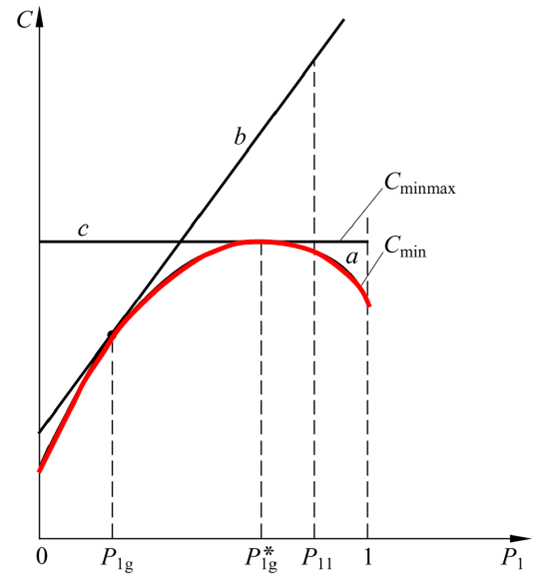
\includegraphics[scale=0.18]{C-P1}
\end{columns}
\end{frame}

\begin{frame}[shrink]
\frametitle{ex6}
\begin{align*}
    P_e&=P(H_1)P(H_0|H_1)+P(H_0)P(H_1|H_0)\\
    &=P(H_1)P_M+P(H_0)P_F\\
    &=[P(H_1)+P(H_0)]P_F &&\text{by }P_M(P_{1g}^\ast)=P_F(P_{1g}^\ast)\\
    &=P_F=P(H_1|H_0) &&\text{by }P(H_1)+P(H_0)=1, P_F\mathop{=}^{def}P(H_1|H_0)\\
    &=Q(\frac{\gamma}{\sigma})=Q\left(\frac{A}{2\sigma}\right) && \text{by }\gamma=\frac{A}{2}\\
    &=Q(\frac{d}{2}) &&\text{by 功率信噪比}d^2=\frac{A^2}{\sigma^2}
\end{align*}
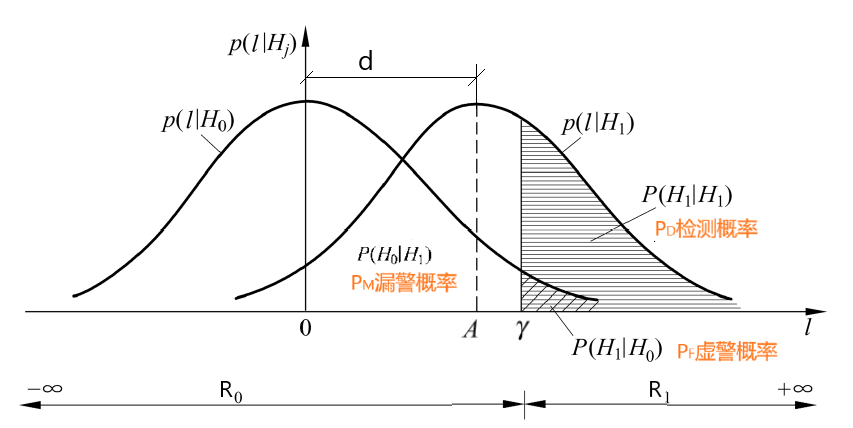
\includegraphics[scale=0.25]{R0R1}
\end{frame}

\begin{frame}
错误判决概率( 虚警概率)$P_F\mathop{=}\limits^{def}P(H_1|H_0)$\textcolor{red}{\textbf{尽可能小}}, 正确判决概率(检测概率)$P_D\mathop{=}\limits^{def}P(H_1|H_1)$\textcolor{red}{\textbf{尽可能大}}。

\medskip 
漏警概率$P(H_0|H_1)+$检测概率$P(H_1|H_1)=1$, 虚警概率$P(H_1|H_0)=\alpha$\\
当$J$最小$\implies$漏警概率$(P(H_0|H_1)$最小$\implies$检测概率$P(H_1|H_1)$最大。

\end{frame}

\begin{frame}{奈曼皮尔逊准则}
\begin{columns}
	\column{0.5\textwidth}
	\begin{enumerate}
		\item 图中,三个判决域$(R_{0i},R_{1i})$均满足错误判决概率$P_i(H_1|H_0)=\alpha(i=0,1,2)$。
		\item 原则上判决域$R_0$和$R_1$有无限多种划分方法,均可以保证错误判决概率$P(H_1|H_0)=\alpha$, 但是正确判决概率$P(H_1|H_1)$一般是不一样的。
		\item 至少有一种判决域划分能使$P(H_1|H_0)=\alpha$,又能使$P(H_1|H_1)$到达最大。
	\end{enumerate}
	\column{0.4\textwidth}
	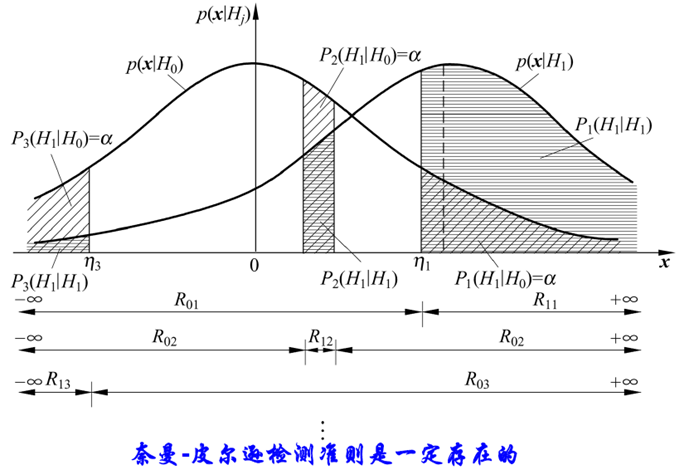
\includegraphics[scale=0.45]{Neyman-Pearson}
\end{columns}
\end{frame}

\begin{frame}{ex3-7}
\textbf{步骤4: 计算判决门限}
\[x\mathop{\gtrless}_{H_0}^{H_1}\sigma^2\ln\mu+\frac{1}{2}\mathop{=}^{def}\gamma \]
在错误判决概率(虚警概率)$P_F\mathop{=}^{def}P(H_1|H_0)=0.1$条件下确定判决门限
\[ P_F\mathop{=}^{def}P(H_1|H_0)=\int_{\gamma}^{\infty}p(x|H_0)dx=\int_{\gamma}^{\infty}\frac{1}{\sqrt{2\pi}}\exp\left(-\frac{x^2}{2}\right)dx=Q(\gamma)=0.1 \]
解得: $\gamma=1.29,\mu=2.2$\\
\begin{columns}
	\column{0.5\textwidth}
	正确判决概率(检测概率):
	\begin{align*}
	P(H_1|H_1)&=\int_{\gamma}^{\infty}\frac{1}{\sqrt{2\pi}}\exp\left[-\frac{(x-1)^2}{2}\right]dx\\
	&=\int_{1.29}^{\infty}\frac{1}{\sqrt{2\pi}}\exp\left[-\frac{(x-1)^2}{2}\right]dx=0.386
	\end{align*}
	\column{0.4\textwidth}
	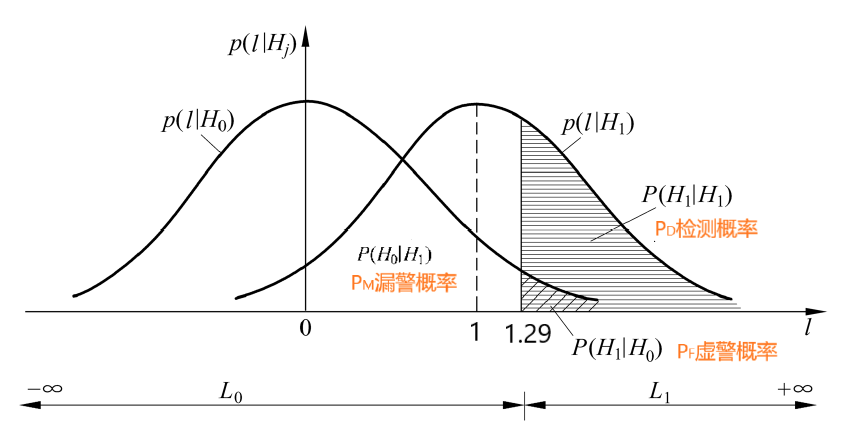
\includegraphics[scale=0.2]{ex3-7}
	\scriptsize
	判决域及判决概念率$P(H_1|H_0)$和$P(H_1|H_1)$
\end{columns}
\end{frame}

\begin{frame}[shrink]
\begin{columns}
	\column{0.5\textwidth}
	检测模型:
	\begin{align*}
	H_0:\quad&x=n\\
	H_1:\quad&x=A+n
	\end{align*}
	似然比检验的判别式:
	\[\frac{1}{N}\sum_{i=1}^{N}x_i\mathop{\gtrless}_{H_0}^{H_1}\frac{\sigma^2\ln\eta}{NA}+\frac{A}{2}\mathop
	{=}^{def}\gamma \]
	统计量$l(x)$:
	\[l(x)\mathop{=}^{def}\frac{1}{N}\sum_{i=1}^{N}x_i \]
	\column{0.4\textwidth}
	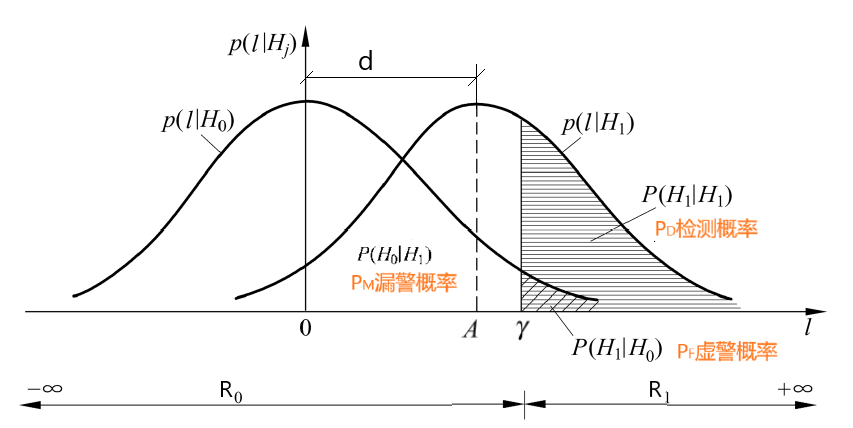
\includegraphics[scale=0.2]{R0R1}
	\scriptsize
	判决域及判决概念率$P(H_1|H_0)$和$P(H_1|H_1)$\\
	\normalsize
	错误判别概率(虚警概率):
	\[P_F=P(H_1|H_0)=Q\left(\frac{\ln\eta}{d}+\frac{d}{2}\right)\]
	正确判别概率(检测概率):
	\[P_D=P(H_1|H_1)=Q\left(\frac{\ln\eta}{d}-\frac{d}{2}\right)\]
	式中$d^2=\frac{NA^2}{\sigma^2}$, 是功率信噪比, $d=\sqrt{N}A/\sigma$, 称为幅度信噪比。
\end{columns}
\end{frame}

\begin{frame}[shrink]
\begin{columns}
	\column{0.6\textwidth}
	\small
    \begin{itemize}
    	\item 似然比检验的判别式:
    	\[\lambda(x)=\frac{p(\bm{x}|H_1)}{p(\bm{x}|H_0)}\mathop{\gtrless}_{H_0}^{H_1}\eta \]
    	\item 错误判别概率(虚警概率):
    	\[P_F=P(H_1|H_0)=Q\left(\frac{\ln\eta}{d}+\frac{d}{2}\right)\]
    	\item 正确判别概率(检测概率):
    	\[P_D=P(H_1|H_1)=Q\left(\frac{\ln\eta}{d}-\frac{d}{2}\right)\]
    	\item 不同的信噪比$d$, 有不同的$P_D\sim P_F$曲线
    	\item 似然比函数$\lambda(x)$超过无穷大门限$\eta=+\infty$是不可能事件, $(P_D,P_F)=(0,0)$
    	\item $\lambda(x)\ge 0$, $\eta=0$是必然事件, $(P_D,P_F)=(1,1)$
    	\item 当$\lambda(x)$是连续随机变量时, $\eta\uparrow\implies (P_D,P_F)\downarrow$
    \end{itemize}
	\column{0.4\textwidth}
	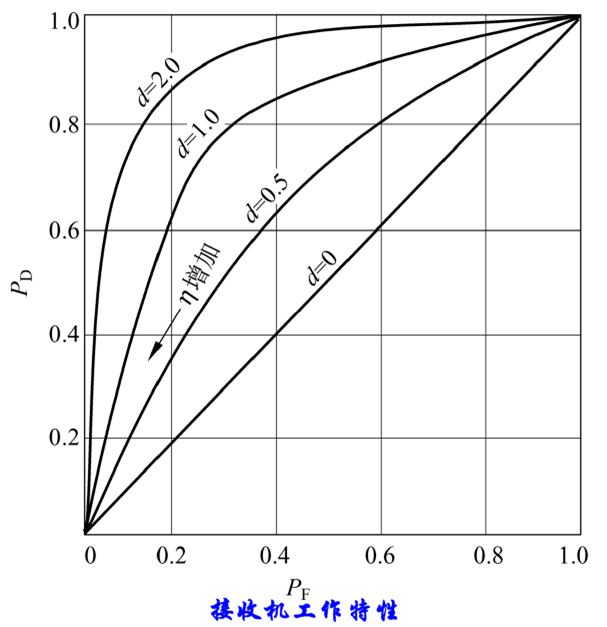
\includegraphics[scale=0.3]{PDPF}\\
	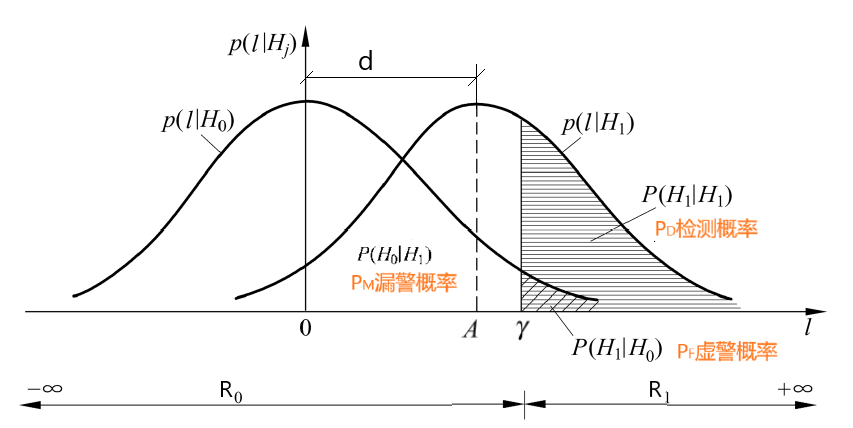
\includegraphics[scale=0.2]{R0R1}
\end{columns}
\end{frame}

\begin{frame}[shrink]
信噪比$d$是接收机的主要指标之一,因此常把接收机工作特性改成$P_D\sim d$曲线, 而以$P_F$作为参变量。
\begin{columns}
	\column{0.4\textwidth}
	\begin{align*}
	P_F&=P(H_1|H_0)=Q(\ln\eta/d+d/2)\\ 
	&\ln\eta/d=Q^{-1}[P(H_1|H_0)]-d/2\\
	P_D&=P(H_1|H_1)=Q\left(\ln\eta/d-d/2\right)\\
	&=Q[Q^{-1}[P(H_1|H_0)]-d/2-d/2]\\
	&=Q[Q^{-1}[P(H_1|H_0)]-d]
	\end{align*}
	\column{0.6\textwidth}
	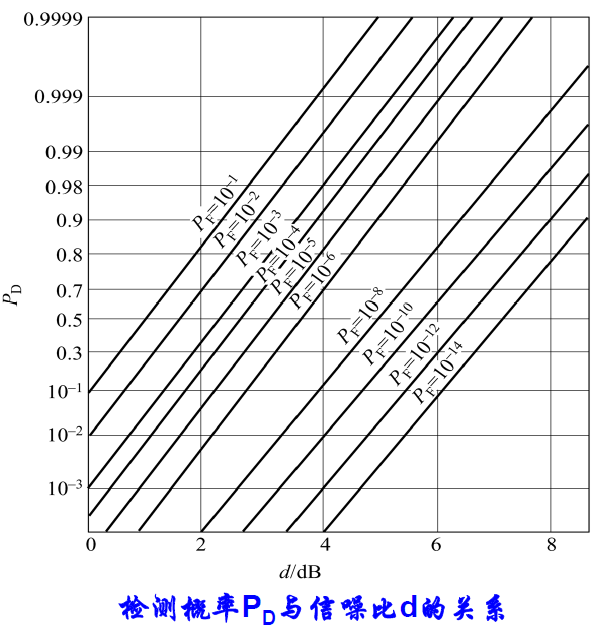
\includegraphics[scale=0.5]{PD-d}
\end{columns}

\medskip

\colorbox{yellow}{$Q(x)$是递减函数, 当给定$P_F$时, $P_D$随功率信噪比$(d^2=NA^2/\sigma^2)$单调增加。} 
\end{frame}

\begin{frame}[shrink]
\begin{align*}
&P_D=P(H_1|H_1)=\int_{\eta}^{\infty}p(\lambda|H_1)d\lambda\mathop{=}^{def}P_D(\eta) \\
&P_F =P(H_1|H_0)=\int_{\eta}^{\infty}p(\lambda|H_0)d\lambda\mathop
{=}^{def}P_F(\eta) \\
&\frac{dP_D(\eta)}{d\eta} =-p(\eta|H_1) \\ 
&\frac{dP_F(\eta)}{d\eta} =-p(\eta|H_0) \\ 
&\qquad \text{ by } \Phi^\prime(x)=\frac{d}{dx}\int_a^xf(t)dt=f(x)\qquad (a\le x\le b) \\
&\frac{dP_D(\eta)}{dP_F(\eta)} =\frac{-p(\eta|H_1)}{-p(\eta|H_0)}=\frac{p(\eta|H_1)}{p(\eta|H_0)}
\end{align*}
\end{frame}

\begin{frame}
\begin{align*}
P_D(\eta) &=P[(\lambda|H_1)\ge\eta]&\\
&=\int_{\eta}^{\infty}p(\lambda|H_1)d\lambda&\\
&=\int_{R_1}^{\infty}p(x|H_1)dx&\\
&=\int_{R_1}^{\infty}\lambda p(x|H_0)dx \qquad \text{ by }\lambda(x)=\frac{p(x|H_1)}{p(x|H_0)}\mathop{\gtrless}_{H_0}^{H_1}\eta&\\
&=\int_{\eta}^{\infty}\lambda p(\lambda|H_0)d\lambda&\\
&\text{ by } \Phi^\prime(x)=\frac{d}{dx}\int_a^xf(t)dt=f(x)\qquad (a\le x\le b) \\
\frac{dP_D(\eta)}{d\eta} &=-\eta p(\eta|H_0)\\
\frac{dP_D(\eta)}{dP_F(\eta)} &=\frac{-p(\eta|H_1)}{-p(\eta|H_0)}=\frac{-\eta p(\eta|H_0)}{-p(\eta|H_0)}=\eta
\end{align*}
\end{frame}

\begin{frame}
\begin{align*}
P_D &\mathop{=}^{def}P_F(P_1)=P(H_1|H_1)\\
P_F &\mathop{=}^{def}P_F(P_1)=P(H_1|H_0)\\
P_M &\mathop{=}^{def}P_M(P_1)=P(H_0|H_1)\\
&=1-P_D
\end{align*}
\[\bm{P_M(P_{1g}^\ast)=1-P_D(P_{1g}^\ast)} \]
\end{frame}

\begin{frame}
$H_1$含随机变量$m$的似然比检验的判别式:
\[\lambda(x)=\frac{p(x|m; H_1)}{p(x|H_0)}=\frac{\int_{-\infty}^{\infty}p(x|m,H_1)p(m)dm}{p(x|H_0)}\mathop{\gtrless}_{H_0}^{H_1}\eta \]
\end{frame}

\begin{frame}
$p(m)$未知
\begin{align*}
&p(x|H_0)=(\frac{1}{2\pi\sigma_n^2})^{1/2}\exp(-\frac{x^2}{2\sigma_n^2})\\
&p(x|m;H_1)=(\frac{1}{2\pi\sigma_n^2})^{1/2}\exp(-\frac{(x-m)^2}{2\sigma_n^2})\\
&\lambda(x)=\frac{p(x|m; H_1)}{p(x|H_0)}\mathop{\gtrless}_{H_0}^{H_1}\eta\\
&\exp(\frac{2mx}{2\sigma_n^2}-\frac{m^2}{2\sigma_n^2})\mathop{\gtrless}_{H_0}^{H_1}\eta\\
&mx\mathop{\gtrless}_{H_0}^{H_1}\sigma_n^2\ln\eta+\frac{m^2}{2}
\end{align*}
\end{frame}

\begin{frame}
\begin{align*}
&m_0\le m\le m_1,m_0>0\\
&mx\mathop{\gtrless}_{H_0}^{H_1}\sigma_n^2\ln\eta+\frac{m^2}{2}\\
&l(x)=x\mathop{\gtrless}_{H_0}^{H_1}\frac{\sigma_n^2}{m}\ln\eta+\frac{m}{2}\mathop{=}^{def}\gamma^+\\
&\int_{\gamma^+}^{\infty}(\frac{1}{2\pi\sigma_n^2})^{1/2}\exp(-\frac{l^2}{2\sigma_n^2})dl=\alpha
\end{align*}
\end{frame}

\begin{frame}
\begin{align*}
&m_0\le m\le m_1,m_1<0\\
&mx\mathop{\gtrless}_{H_0}^{H_1}\sigma_n^2\ln\eta+\frac{m^2}{2}\\
&l(x)=x\mathop{\lessgtr}_{H_0}^{H_1}-\frac{\sigma_n^2}{|m|}\ln\eta-\frac{|m|}{2}\mathop{=}^{def}\gamma^-\\
&\int_{-\infty}^{\gamma^-}(\frac{1}{2\pi\sigma_n^2})^{1/2}\exp(-\frac{l^2}{2\sigma_n^2})dl=\alpha
\end{align*}
\end{frame}

\begin{frame}
若$m_0>0$, $m$仅取正值, 则在$P(H_1|H_0)=\alpha$的约束下, $P^{(m)}(H_1|H_1)$是最大的,其一致最大功效检验成立;\\
若$m_1<0$, $m$仅取负值, 则在$P(H_1|H_0)=\alpha$的约束下, $P^{(m)}(H_1|H_1)$也是最大的。
\end{frame}

\begin{frame}
若$m_0<0,m_1>0$, 即$m$取值可能为正或可能为负的情况下, 无论参量信号的统计检测,按$m$仅取正值设计,还是按$m$仅取负值设计,都有可能在某些$m$值下,   $P^{(m)}(H_1|H_1)$不满足最大的要求。\\
例如,按$m$取正设计信号检测系统,当$m$为正时,$P^{(m)}(H_1|H_1)$最大, 但当$m$为负时, $P^{(m)}(H_1|H_1)$可能最小。\\
因此, 这种情况下不能采用奈曼-皮尔逊准则来实际最佳检测系统。
\end{frame}

\begin{frame}
若$m_0<0,m_1>0$, 即$m$取值可能为正或可能为负,奈曼-皮尔逊准则不能保证$P^{(m)}(H_1|H_1)$最大要求。考虑把约束条件$P(H_1|H_0)=\alpha$分成两个$\alpha/2$, 假设$H_1成立$的判决域由两部分组成。判决表示式为
	\[|x|\mathop{\gtrless}_{H_0}^{H_1}\gamma \]

\begin{block}{}
	虽然双边检验比均值$m$假定为正确时的单边检验性能差,但是比均值$m$假定为错误时的单边检验性能要好的多。因此不失为一种好的折中方法。
\end{block}
\end{frame}

\begin{frame}{广义似然比检验}
\begin{align*}
&\text{似然函数}\\
&p(x|m;H_1)=(\frac{1}{2\pi\sigma_n^2})^{1/2}\exp(-\frac{(x-m)^2}{2\sigma_n^2})\\
&\text{对$m$求偏导,令结果等于零,即} \\
&\frac{\partial\ln p(x|m;H_1)}{\partial m}|_{m=\widehat{m}_{ml}}=0\\
&\text{解得单次观测时,$m$的最大似然估计量$\widehat{m}_{ml}=x$, 于是有 }\\
&p(x|\widehat{m}_{ml};H_1)=(\frac{1}{2\pi\sigma_n^2})^{1/2}\exp(-\frac{(x-\widehat{m}_{ml})^2}{2\sigma_n^2})|_{\widehat{m}_{ml}=x}=(\frac{1}{2\pi\sigma_n^2})^{1/2}\\
\end{align*}
\end{frame}
\begin{frame}{广义似然比检验}
\begin{align*}
&p(x|H_0)=(\frac{1}{2\pi\sigma_n^2})^{1/2}\exp(-\frac{x^2}{2\sigma_n^2})
&p(x|\widehat{m}_{ml};H_1)=(\frac{1}{2\pi\sigma_n^2})^{1/2}\\
&\text{代入广义似然比检验中, 有}\\
&\lambda(x)=\frac{p(x|m; H_1)}{p(x|H_0)}\mathop{\gtrless}_{H_0}^{H_1}\eta\\
&\lambda(x)=\frac{(\frac{1}{2\pi\sigma_n^2})^{1/2}}{(\frac{1}{2\pi\sigma_n^2})^{1/2}\exp(-\frac{x^2}{2\sigma_n^2})}\mathop{\gtrless}_{H_0}^{H_1}\eta\\
&\text{化简得判决表示式}
&x^2\mathop{\gtrless}_{H_0}^{H_1}2\sigma_n^2\ln\eta\mathop{=}^{def}\gamma^2 \implies |x|\mathop{\gtrless}_{H_0}^{H_1}\gamma
\end{align*}
这正是前面讨论过的双边检验。只是前面是从奈曼-皮尔逊准则出发推导得到。而这里是从似然比检验的概念导出的,似然函数$p(x|m;H_1)$中的信号参量$m$由其最大似然估计量$\widehat{m}_{ml}$代换,所以是广义似然比检验。
\end{frame}

\begin{frame}{title}
\begin{align*}
H_0&=-A+n\\
H_1&=A+n\\
p(n)&=\left(\frac{1}{2\pi\sigma^2}\right)^{1/2}\exp\left[-\frac{n^2}{2\sigma^2}\right]\\
p(x|H_0)&=\left(\frac{1}{2\pi\sigma^2}\right)^{1/2}\exp\left[-\frac{(x+A)^2}{2\sigma^2}\right]\\
p(x|H_1)&=\left(\frac{1}{2\pi\sigma^2}\right)^{1/2}\exp\left[-\frac{(x-A)^2}{2\sigma^2}\right]
\end{align*}
\end{frame}

\begin{frame}{title}
\begin{itemize}
	\item 目标: 正确判决概率$P(H_j|H_j)$尽可能大,错误判决概率$P(H_i|H_j)(i\ne j)$尽可能小。
	\item $x_0\downarrow\implies P(H_1|H_1)\uparrow$, 但$P(H_0|H_1)\downarrow$。如果$x_0\uparrow$,结果相反。
	\item 因此需要最佳划分判决域
\end{itemize}
\end{frame}




